\chapter[AGES IV --- Estudify]{AGES IV --- ESTUDIFY}

Este capítulo apresenta a passagem do aluno como \ac{ages} IV pelo Projeto Estudify. Aqui estão descritos os artefatos entregues, a atuação ao longo das sprints e os pontos de melhoria identificados.

\section[Introdução]{Introdução}

O projeto foi concebido a partir de uma ``dor'' identificada pelas \textit{stakeholders} Eliza Pasquali Lunardi e Letícia Fossá Rosa, fundadoras do Estudify e vencedoras do Startup Garagem. Embora já possuíssem uma plataforma web funcional de preparação para o ENEM e vestibulares com usuários pagantes, as clientes enfrentavam limitações na experiência oferecida aos estudantes e dificuldades recorrentes na gestão de conteúdo, identificando a necessidade de evoluir o produto para uma aplicação \textit{mobile} nativa, mais engajadora e alinhada ao comportamento do público jovem.

O projeto teve como objetivo tornar o estudo para o ENEM e vestibulares mais leve e eficiente, por meio de uma experiência gamificada inspirada no Duolingo. Foi proposto um aplicativo \textit{mobile} em que o estudante aprende resolvendo questões organizadas por disciplina e tópico, com \textit{feedback} instantâneo via gabarito comentado, complementado por simulados completos no formato ENEM, cronograma personalizado de estudos e um sistema de gamificação com moedas, \textit{streaks} diários e acompanhamento de progresso. O projeto também contemplou um painel administrativo web, destinado às clientes, para importação em lote de questões e acompanhamento dos usuários.

A execução do projeto ocorreu no primeiro semestre de 2026, entre os dias 02 de março e 29 de junho de 2026, compreendendo diversas etapas realizadas pelos estudantes do bacharelado em Engenharia de Software no âmbito da \ac{ages}, sob a orientação do professor Marcelo H. Yamaguti. A foto do time responsável pelo projeto pode ser vista na Figura~\ref{fig:estudify-time}.

\begin{figure}[H]
    \centering
    \small
    \caption{Time do projeto Estudify}
    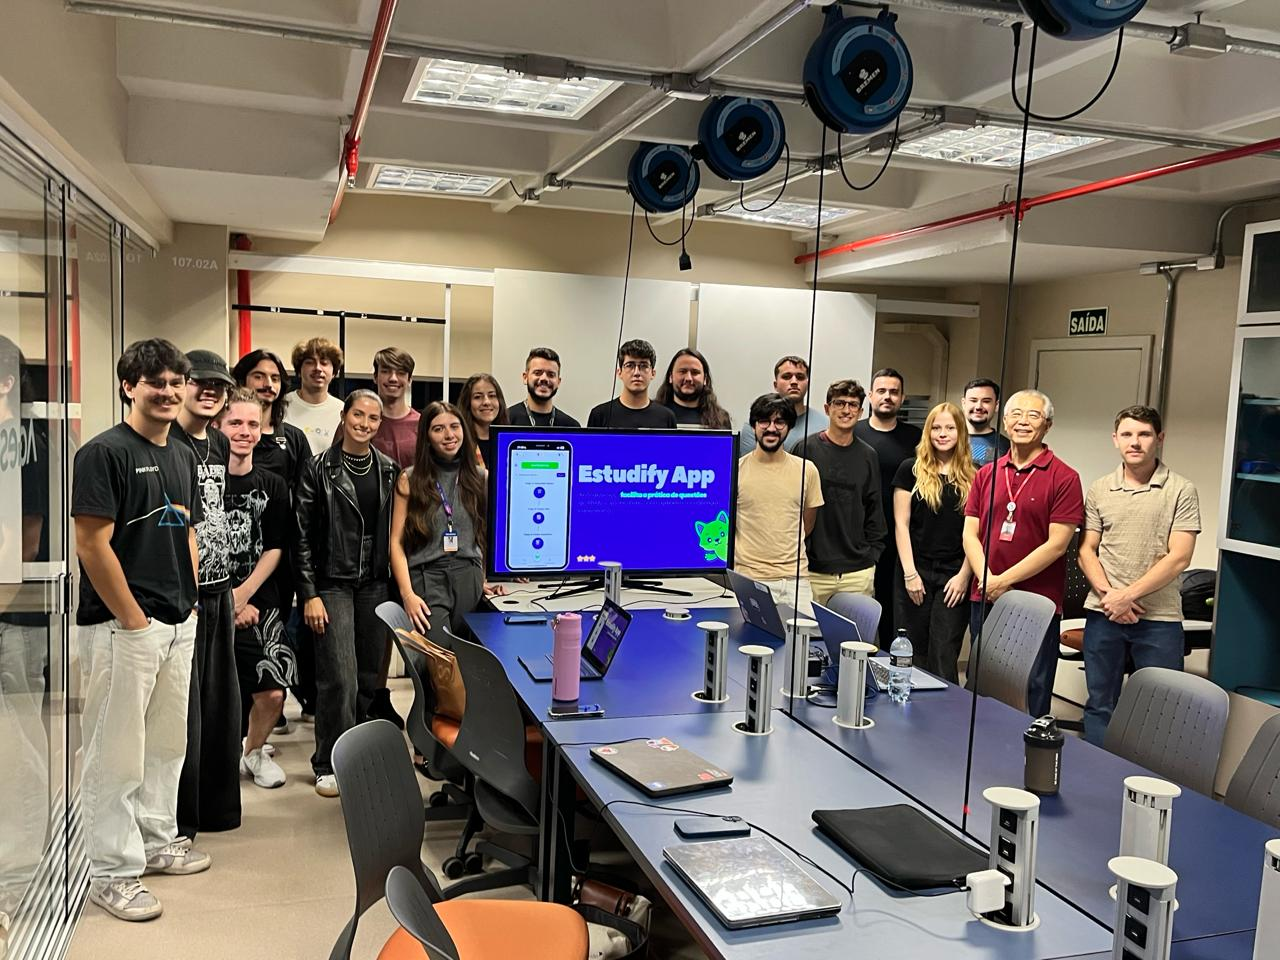
\includegraphics[width=0.9\linewidth]{conteudo/5 - ages IV/images/fig11-time-estudify.png}

    Fonte: Wiki do projeto
    \label{fig:estudify-time}
\end{figure}

\section[Desenvolvimento do Projeto]{Desenvolvimento do Projeto}

Esta seção apresenta informações relativas ao desenvolvimento do projeto: localização do código-fonte e documentação, arquitetura e tecnologias utilizadas, e protótipos de tela desenvolvidos. Toda a documentação do projeto pode ser encontrada na wiki do mesmo: \url{https://tools.ages.pucrs.br/estudify/estudify-wiki/-/wikis/home}.

\subsection{Repositório do Código Fonte do Projeto}
  Todo o código do projeto encontra-se distribuído em três repositórios:
\begin{itemize}
    \item código do \textit{frontend} web: \url{https://tools.ages.pucrs.br/estudify/frontend-web};
    \item código do \textit{frontend} \textit{mobile}: \url{https://tools.ages.pucrs.br/estudify/frontend-mobile};
    \item código do \textit{backend}: \url{https://tools.ages.pucrs.br/estudify/backend}.
\end{itemize}

\subsection{Banco de Dados Utilizado}
  O banco de dados escolhido foi o PostgreSQL, um banco de dados transacional que possui todas as propriedades ACID. Com isso, garante a segurança das transações, sejam elas concorrentes ou não, mantendo o seu estado inalterado mesmo frente a falhas, além de garantir a aplicação total das operações.

  Foi desenvolvido de maneira relacional, o que facilitou o tratamento dos relacionamentos entre as entidades da aplicação, como mostra o esquema conceitual desenvolvido, na Figura~\ref{fig:estudify-mc}.

\begin{figure}[H]
    \centering
    \small
    \caption{Modelo Conceitual Estudify}
    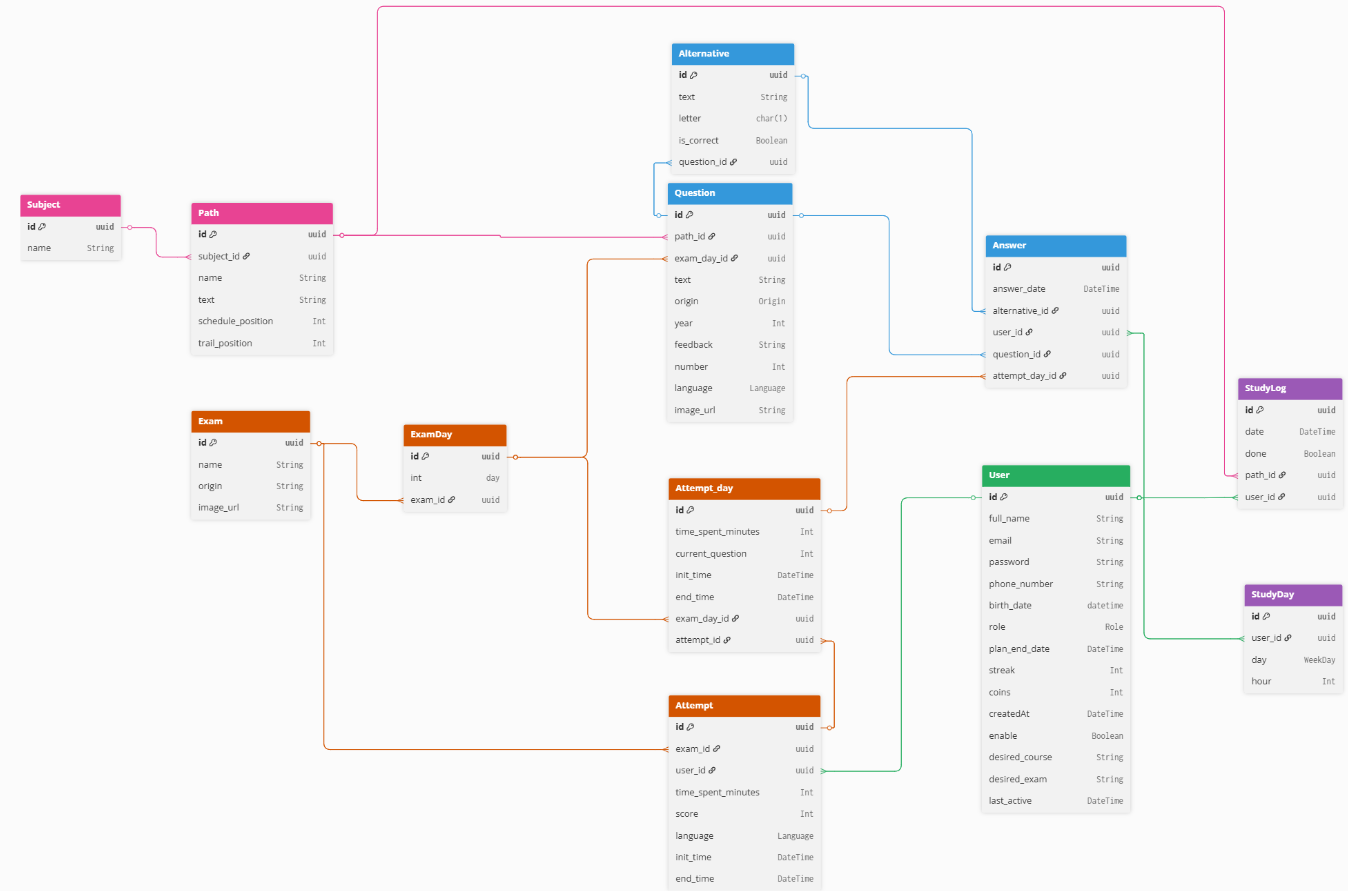
\includegraphics[width=0.9\linewidth]{conteudo/5 - ages IV/images/fig12-modelo-conceitual.png}

    Fonte: Wiki do projeto
    \label{fig:estudify-mc}
\end{figure}

\subsection{Arquitetura Utilizada}
  A arquitetura do projeto segue o padrão de Monólito Modular no \textit{back-end}, em que as funcionalidades são segregadas por domínio. Cada módulo é composto por \textit{Controllers}, responsáveis pelas rotas e requisições HTTP; \textit{Services}, que concentram as regras de negócio; \textit{Repositories}, camada isolada de comunicação com o banco de dados; e \ac{dto} (\textit{Data Transfer Objects}), que definem os contratos de entrada com validações integradas.

  A aplicação \textit{mobile} e o painel administrativo web adotam uma estrutura de pastas análoga entre si (\textit{components}, \textit{hooks}, \textit{services} e \textit{contexts}), mantendo a consistência técnica entre as frentes e permitindo que qualquer integrante do time atue em ambas.

  O fluxo de comunicação entre as camadas está ilustrado no diagrama da Figura~\ref{fig:estudify-fluxo}, evidenciando a separação entre os clientes (\textit{mobile} e web), a API e o banco de dados.

\begin{figure}[H]
    \centering
    \small
    \caption{Diagrama de fluxo da aplicação}
    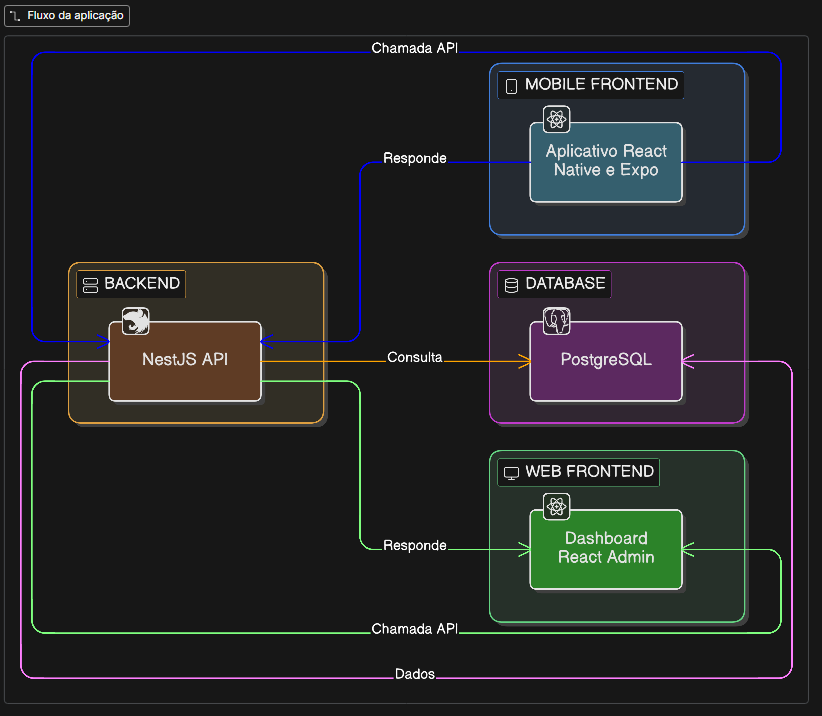
\includegraphics[width=0.9\linewidth]{conteudo/5 - ages IV/images/fig13-diagrama-fluxo.png}

    Fonte: Wiki do projeto
    \label{fig:estudify-fluxo}
\end{figure}

\subsection{Protótipos das Telas Desenvolvidas}
  Os protótipos deste projeto estão disponíveis na wiki do projeto: \url{https://tools.ages.pucrs.br/estudify/estudify-wiki/-/wikis/design}.

  A Figura~\ref{fig:estudify-prototipos} apresenta uma amostra das telas do aplicativo, contemplando os principais fluxos do usuário: o acompanhamento do progresso com os elementos de gamificação, a tela de treino com a seleção de disciplinas e tópicos, a resolução de questões e o respectivo \textit{feedback} com a explicação da resposta, além do \textit{onboarding} de primeiro acesso e da tela de perfil.

\begin{figure}[H]
    \centering
    \small
    \caption{Protótipos das telas do aplicativo \textit{mobile}}
    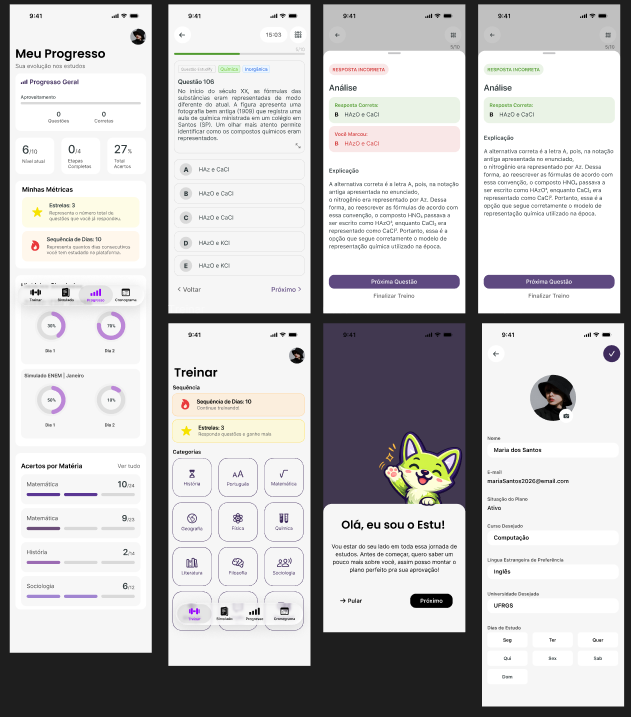
\includegraphics[width=0.9\linewidth]{conteudo/5 - ages IV/images/fig14-prototipos.png}

    Fonte: Wiki do projeto
    \label{fig:estudify-prototipos}
\end{figure}

  Além do aplicativo \textit{mobile}, o projeto conta com um painel administrativo web, destinado à gestão de conteúdo da plataforma. As Figuras \ref{fig:estudify-admin-questoes}, \ref{fig:estudify-admin-simulados} e \ref{fig:estudify-admin-importacao} apresentam as principais telas desse painel. A Figura~\ref{fig:estudify-admin-questoes} exibe a tela de gestão de questões, com busca, filtro por categoria e a listagem de todas as questões cadastradas. A Figura~\ref{fig:estudify-admin-simulados} apresenta a tela de gestão de simulados, em que é possível organizar os simulados e definir a ordem das questões que os compõem. Por fim, a Figura~\ref{fig:estudify-admin-importacao} mostra a tela de revisão das questões importadas em lote via CSV, sinalizando o \textit{status} de cada uma (sucesso, falta de imagem ou erro) para que os ajustes necessários sejam feitos antes da confirmação.

\begin{figure}[H]
    \centering
    \small
    \caption{Painel administrativo: gestão de questões}
    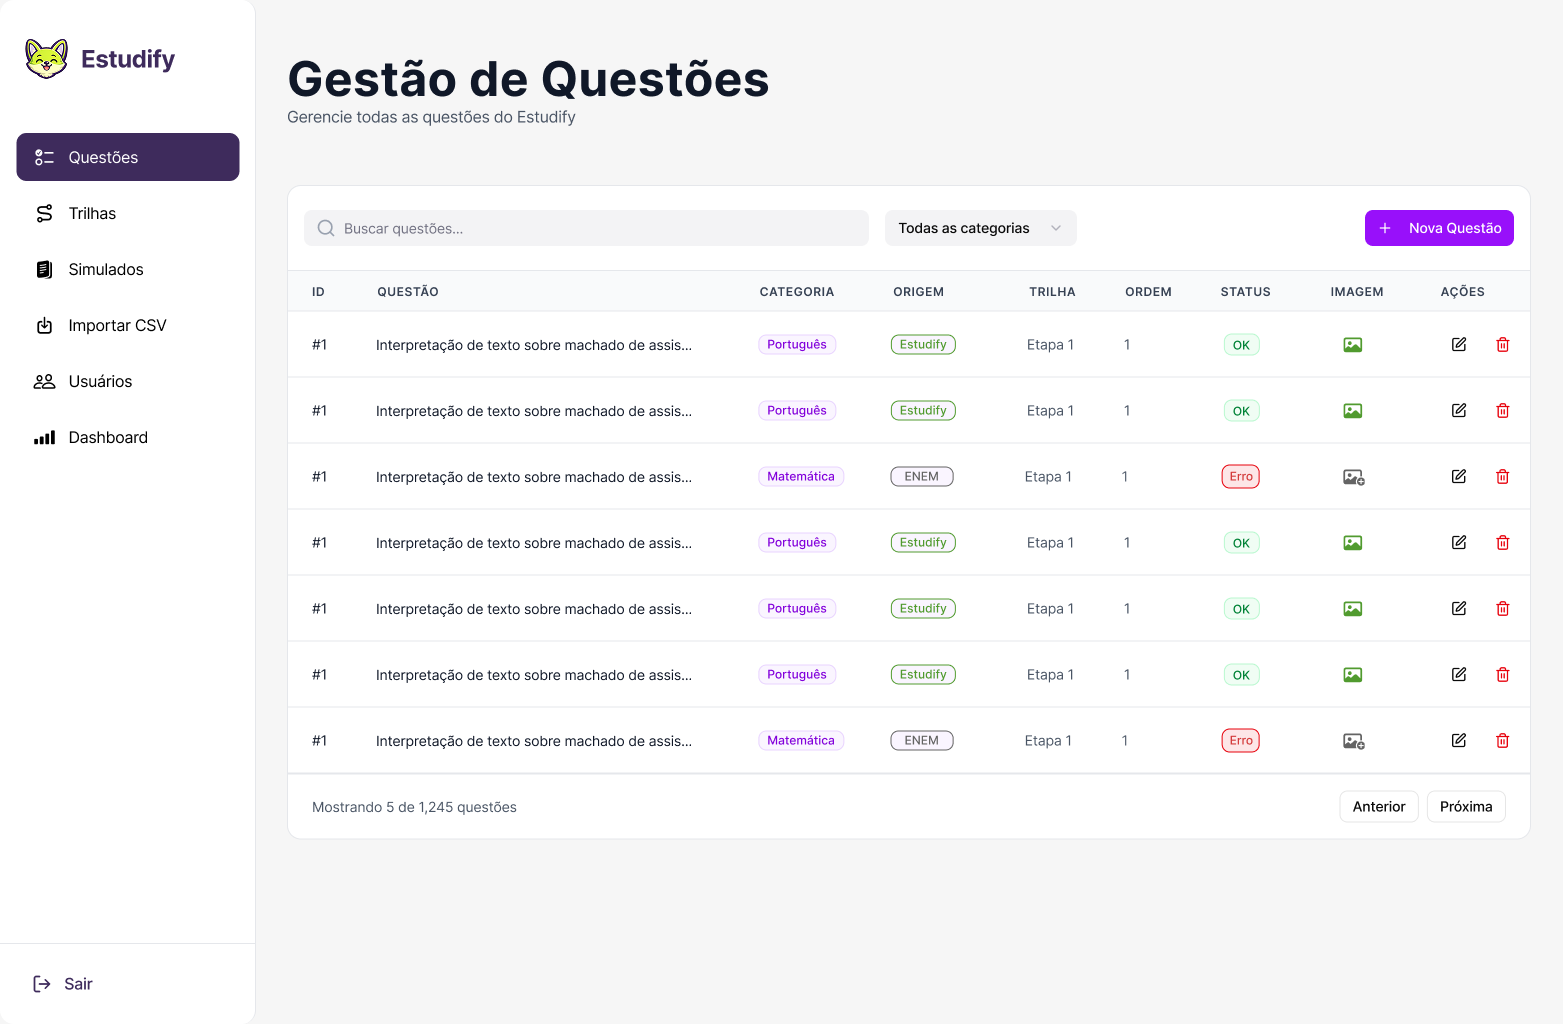
\includegraphics[width=0.7\linewidth]{conteudo/5 - ages IV/images/fig15-admin-questoes.png}

    Fonte: Wiki do projeto
    \label{fig:estudify-admin-questoes}
\end{figure}

\begin{figure}[H]
    \centering
    \small
    \caption{Painel administrativo: gestão de simulados}
    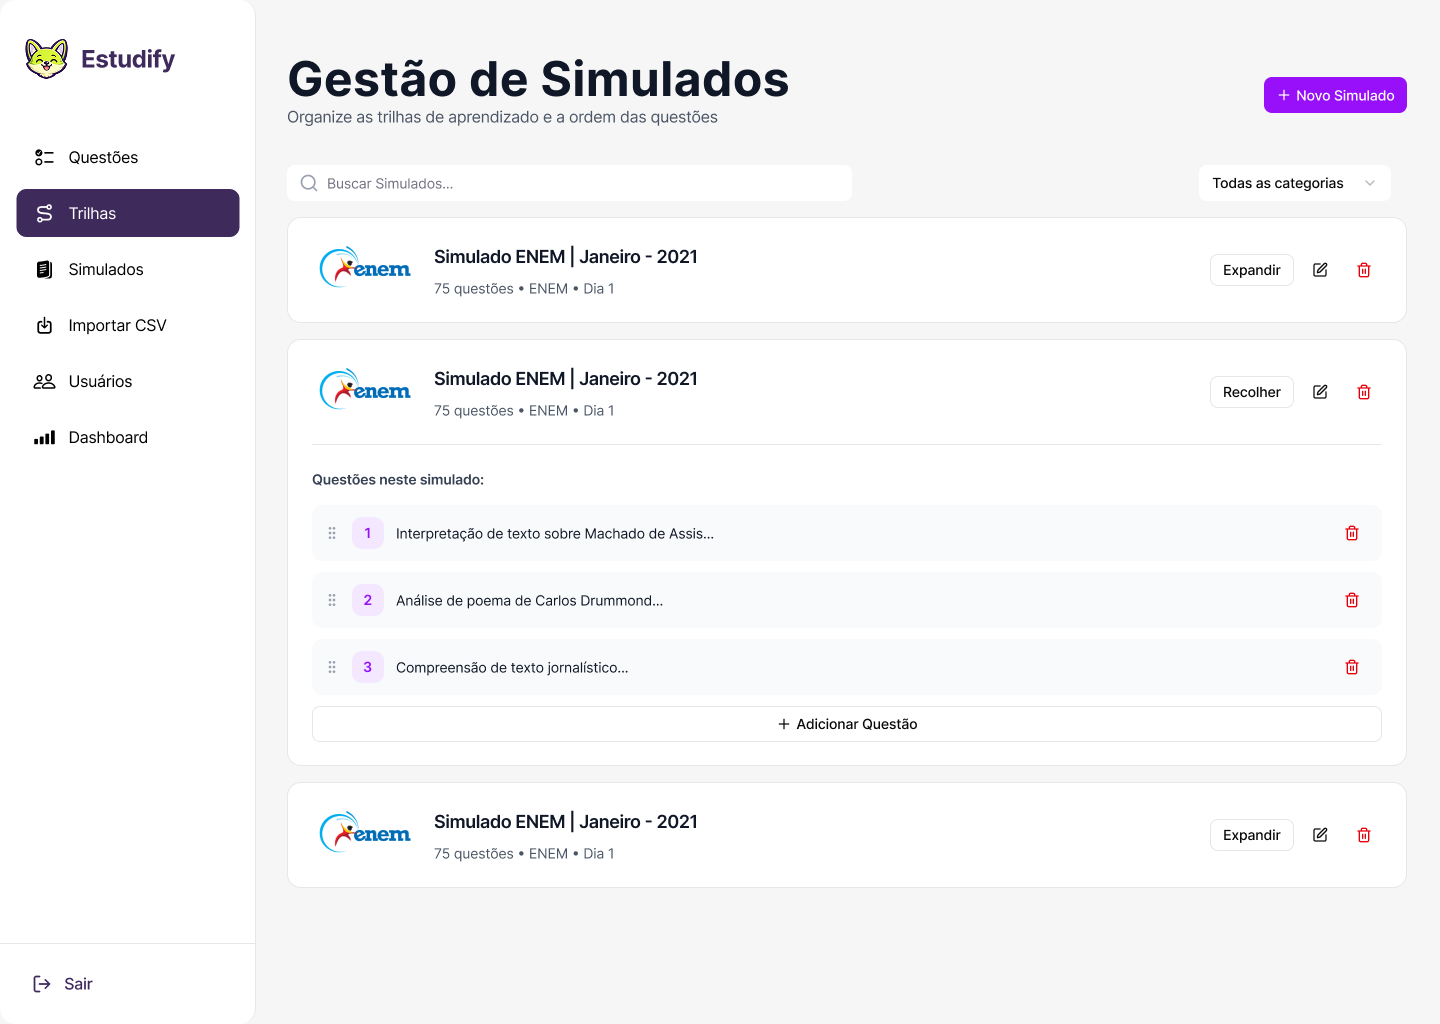
\includegraphics[width=0.7\linewidth]{conteudo/5 - ages IV/images/fig16-admin-simulados.png}

    Fonte: Wiki do projeto
    \label{fig:estudify-admin-simulados}
\end{figure}

\begin{figure}[H]
    \centering
    \small
    \caption{Painel administrativo: revisão de questões importadas via CSV}
    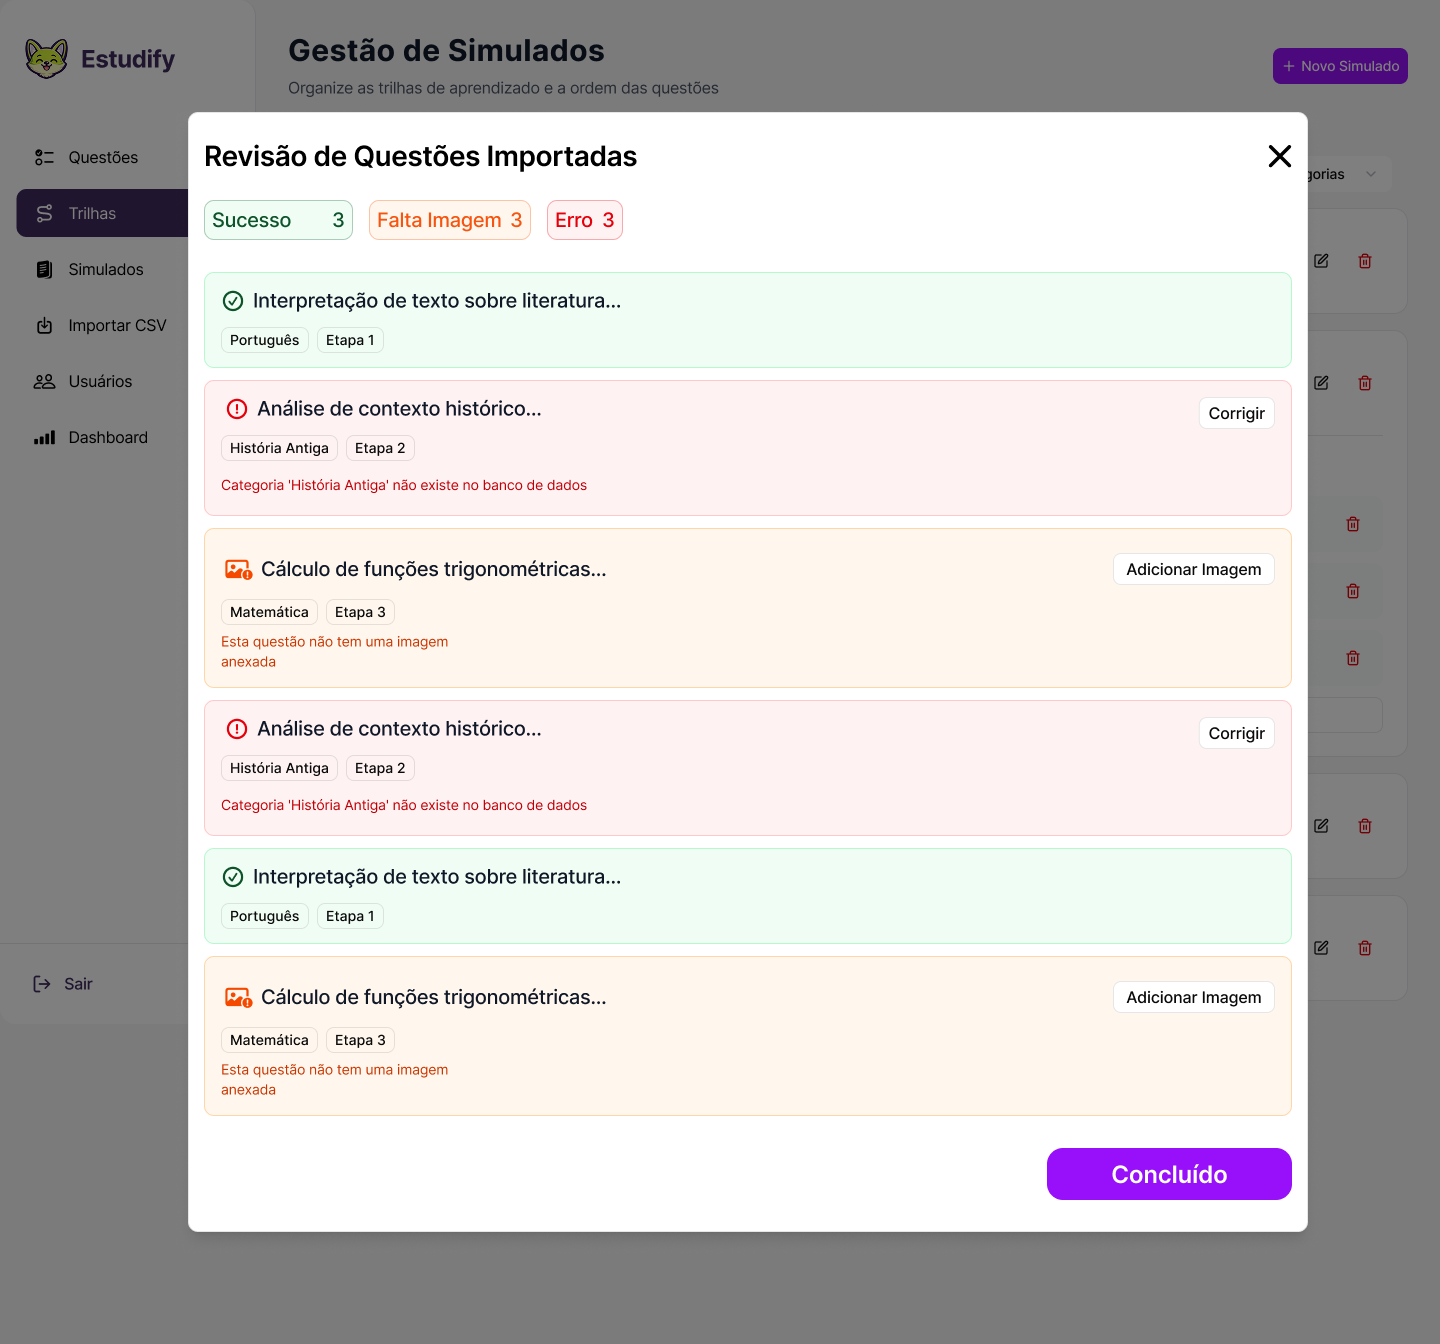
\includegraphics[width=0.55\linewidth]{conteudo/5 - ages IV/images/fig17-admin-importacao.png}

    Fonte: Wiki do projeto
    \label{fig:estudify-admin-importacao}
\end{figure}

\subsection{Tecnologias Utilizadas}
  Nesta seção serão apresentadas as principais tecnologias empregadas no desenvolvimento do projeto Estudify, destacando suas contribuições para o sucesso da implementação. As ferramentas estão organizadas conforme a camada da aplicação em que foram utilizadas.

\begin{itemize}
    \item \textbf{TypeScript} \parencite{typescript}: \textit{Superset} do JavaScript que adiciona tipagem estática opcional, reduzindo \textit{bugs} em tempo de desenvolvimento e facilitando a manutenção do código. Foi adotado como linguagem base em todas as camadas da aplicação (\textit{back-end}, \textit{mobile} e web), permitindo o compartilhamento de tipos e interfaces entre as frentes do projeto.
    \item \textbf{Node.js} \parencite{nodejs}: Ambiente de execução JavaScript \textit{server-side} com natureza assíncrona e eficiência no gerenciamento de I/O, ideal para o processamento de múltiplas requisições simultâneas. Serve como base para a execução do NestJS.
    \item \textbf{NestJS} \parencite{nestjs}: \textit{Framework} progressivo para Node.js que permite a construção de aplicações escaláveis com arquitetura modular e suporte nativo a TypeScript. Foi utilizado na construção da API do projeto, oferecendo recursos como injeção de dependência, \textit{decorators} e validação integrada de \ac{dto}.
    \item \textbf{Prisma} \parencite{prisma}: \ac{orm} (\textit{Object-Relational Mapper}) que atua como ponte entre a aplicação e o banco de dados relacional. Gera tipos automaticamente a partir do \textit{schema} do banco, garantindo \textit{type-safety} nas consultas, além de simplificar a criação e execução de \textit{migrations}.
    \item \textbf{PostgreSQL} \parencite{postgresql}: Sistema de gerenciamento de banco de dados relacional \textit{open source} que implementa as propriedades ACID, garantindo a integridade e a consistência dos dados armazenados. Escolhido por sua robustez, confiabilidade e maturidade no mercado.
    \item \textbf{React Native} \parencite{reactnative}: \textit{Framework} para desenvolvimento de aplicações \textit{mobile} nativas a partir de uma única base de código em TypeScript, permitindo a entrega simultânea para iOS e Android. Foi utilizado na construção do aplicativo principal do Estudify.
    \item \textbf{Expo} \parencite{expo}: Plataforma e ecossistema construído sobre o React Native que agiliza o desenvolvimento \textit{mobile}, fornecendo ferramentas integradas de \textit{build}, execução e distribuição, além do Expo Router para roteamento baseado em arquivos.
    \item \textbf{React} \parencite{react}: Biblioteca JavaScript de código aberto para construção de interfaces de usuário reativas e componentes reutilizáveis. Foi utilizada no desenvolvimento do painel administrativo web, destinado à gestão de conteúdo e acompanhamento dos usuários.
\end{itemize}

\section[Atividades Desempenhadas Pelo Aluno no Projeto]{Atividades Desempenhadas Pelo Aluno no Projeto}

Nesta seção será abordada a minha contribuição para o projeto ao longo das \textit{sprints}.

\subsection{\textbf{Sprint 0}}

O projeto teve início com uma reunião com as \textit{stakeholders} Eliza Pasquali Lunardi e Letícia Fossá Rosa, onde tivemos a oportunidade de entender com mais profundidade do que se tratava o Estudify. Nesse encontro, tiramos dúvidas de escopo e prioridades, e alguns ajustes importantes emergiram em relação ao material de abertura do projeto: a revisão de redação, que constava como item do escopo, acabou ficando de fora, enquanto a página web de administração, inicialmente listada como fora do escopo, foi incorporada. Saímos da reunião com bastante material para trabalhar ao longo da \textit{sprint}.

Logo em seguida, nos reunimos entre os \ac{ages} IV para alinhar como conduziríamos o projeto. Já no primeiro dia, debatemos alguns princípios que nortearam toda a nossa atuação. Definimos que as \textit{tasks} seriam escritas de forma bem mais detalhada do que o padrão --- uma decisão baseada no nosso histórico na \ac{ages}, que mostrava que tarefas mal definidas designadas a \ac{ages} I ou II tendiam a gerar retrabalho significativo. Também definimos que trabalharíamos organizados em \textit{squads}, compostas por pelo menos um integrante de cada senioridade, e que cada \ac{ages} IV ficaria responsável por acompanhar uma delas, com a missão de garantir que o time avançasse nas entregas. Essa divisão nos deu um controle muito mais assertivo sobre o andamento do projeto.

Para fundamentar a escolha do \textit{stack}, elaboramos uma pesquisa interna mapeando as tecnologias mais familiares ao time. Deixamos claro desde o início que a decisão final caberia aos \ac{ages} III, por serem eles os responsáveis pela arquitetura. Após a discussão técnica, definiu-se React Native para o \textit{mobile} e NestJS para o \textit{backend}; em conversa com os \ac{ages} II, que responderiam pelo banco, fechamos em PostgreSQL.

Quando conversamos com os \ac{ages} III sobre a distribuição de responsabilidades na \textit{sprint}, dois deles, Eduardo Camana e Isadora Guerra, manifestaram interesse em se dedicar inteiramente à prototipação. Ambos vinham do Apple Academy, e como eu já havia tido experiências muito positivas com a prototipação de quem participa deste programa, decidimos aceitar. Ainda assim, abrimos o convite para qualquer outro integrante do time que quisesse aprender mais sobre essa frente se juntar a eles. Os três \ac{ages} III restantes assumiram a montagem da infraestrutura. Esse tipo de paralelismo só foi viável porque tínhamos cinco \ac{ages} III, um número acima da média para projetos da \ac{ages}, e uma equipe muito engajada no geral.

Em paralelo, estruturamos o escopo do aplicativo em nove épicos, cada um agrupando um conjunto coeso de \ac{us}. Fiquei responsável por escrever as \ac{us} de dois deles: o Épico 3, que concentrava o \textit{core} do produto, toda a jornada de resolução de questões, e o Épico 6, referente à gamificação do aplicativo como um todo. Reforçamos entre nós a disciplina de escrever \textit{tasks} o mais detalhadas possível, com critérios de aceite claros e contratos bem definidos entre \textit{front} e \textit{back}. Quando terminamos de redigir as histórias, nos reunimos como \ac{ages} IV e revisamos uma a uma, garantindo que cada ponto mapeado no escopo tivesse ao menos uma \textit{task} correspondente no ClickUp.

Um ponto que não previmos foi o ritmo de entrega dos \ac{ages} II no modelo de banco. Nossa expectativa era de que um modelo minimamente concreto só apareceria por volta do meio da \textit{Sprint} 1, e estruturamos a escrita das \ac{us} partindo dessa premissa. Os \ac{ages} II, no entanto, conseguiram entregar um modelo bastante completo já no fim da \textit{Sprint} 0, o que, apesar de ser um ótimo resultado de engajamento da equipe, fez com que algumas das histórias que escrevemos ficassem ligeiramente desalinhadas em relação ao modelo que chegou. Não foi um erro muito significativo, mas gerou um ruído extra no início da \textit{Sprint} 1 que poderia ter sido evitado. Ficou como aprendizado, para mim como \ac{ages} IV, a necessidade de sincronizar mais de perto a escrita das \ac{us} com o avanço da modelagem de dados, inclusive nos cenários em que o time técnico entrega acima do esperado, o descompasso pode vir pelos dois lados.

Na apresentação de fechamento da \textit{sprint}, as \textit{stakeholders} ficaram bastante satisfeitas com os protótipos no geral; o resultado foi muito além do que haviam imaginado. Solicitaram apenas alguns ajustes pontuais na \ac{ui}, como trocar a fonte por uma com traços mais arredondados e deixar as telas mais coloridas. Ficaram também de nos enviar alguns ícones que gostariam de ver aplicados no aplicativo, bem como uma lista de questões já existentes no banco de dados delas, que serviria de base para o conteúdo inicial.

Ao final da \textit{sprint}, senti que o time em geral fez um excelente trabalho. O único ponto de atenção que levantei junto aos outros \ac{ages} IV foi que os \ac{ages} I acabaram tendo pouca participação nessa \textit{sprint}: como normalmente são eles que contribuem com os \textit{mockups} nessa fase, e essa frente ficou a cargo do Eduardo e da Isadora, sobrou menos espaço de atuação para eles. Não foi um problema de engajamento, mas algo a observar nas próximas \textit{sprints} para garantir que essa senioridade tenha frentes claras em que possa contribuir.

\subsection{\textbf{Sprint 1}}

Após a apresentação com as \textit{stakeholders}, reunimos o time para dividir as \textit{squads}. Para esta \textit{sprint}, planejamos doze tarefas de desenvolvimento, sendo seis referentes ao Épico 3, de questões, e seis distribuídas entre os demais épicos. Como o número de entregas era menor que o de integrantes, algumas delas acabaram sendo feitas em dupla, normalmente com um \ac{ages} I e um \ac{ages} II trabalhando juntos. O meu time ficou responsável pelas tarefas de autenticação e cadastro do usuário. A distribuição das histórias dentro de cada \textit{squad} ficou a cargo do \ac{ages} IV responsável por ela.

Um detalhe importante é que, antes mesmo do início da \textit{sprint}, um dos \ac{ages} III já havia adiantado a parte de autenticação no \textit{backend}, cobrindo tanto o login quanto o cadastro do usuário. Isso fez com que essa frente já chegasse praticamente concluída na minha \textit{squad}. Entreguei para o \ac{ages} II do time a tarefa de \textit{frontend} de cadastro, e para o \ac{ages} I o carrossel de primeiro acesso ao aplicativo. Como meu \ac{ages} III já tinha adiantado parte do \textit{backend}, optei por passar a ele uma atividade menos complexa, o que permitiria que ele apoiasse os \ac{ages} menores, revisasse os \ac{pr} e começasse a desenhar o diagrama da \ac{aws}, uma entrega que precisaria sair o quanto antes.

Logo após a primeira aula da \textit{sprint}, percebemos que o engajamento do time estava bastante alto. Já havia \ac{pr} abertos para a \textit{develop} nos primeiros dias. Com a capacidade sobrando, começamos a puxar histórias da \textit{Sprint} 3, já que boa parte das entregas da \textit{Sprint} 2 dependia diretamente de cadastro, login e questões ainda em andamento na \textit{Sprint} 1. Antecipar histórias da \textit{Sprint} 3 era mais seguro, pois elas tinham menos acoplamento com o que estava sendo construído naquele momento.

No meu time, no entanto, notei que as coisas andavam um pouco mais devagar, especialmente na tarefa do \ac{ages} II, que estava enfrentando dificuldades com o próprio Git. Conversei individualmente com cada integrante da \textit{squad} para entender se havia algo em que eu pudesse ajudar. Todos responderam que estava tudo certo e que as atividades estavam encaminhadas.

Na aula seguinte, conversei com a \ac{ages} I da \textit{squad} e ela me disse que a tarefa dela estava pronta, mas que tinha dúvida se deveria subir mesmo faltando uma rota. No fim, a rota dependia de uma tela de outra \textit{squad} que acabou atrasando, o que bloqueou parcialmente a entrega dela, ainda que a parte que cabia à \ac{ages} I já estivesse pronta. Já o \ac{ages} II tinha um \ac{pr} aberto com comentários dos \ac{ages} III pedindo ajustes, todos pontuais e resolvidos em aula. A única pendência real que ficou foi a história do \ac{ages} III do time, que acabou atrasando. Como era uma entrega importante, o componente de navegação do aplicativo, que destravaria várias atividades futuras, pedi que outro \ac{ages} III pegasse a tarefa antes do \textit{code freeze}, que havíamos estipulado para uma semana antes da apresentação. O Gabriel Saldanha, de outra \textit{squad}, puxou a história para si e conseguiu finalizá-la faltando três dias para a apresentação, já dentro do \textit{code freeze}.

Na aula anterior à apresentação, tentamos rodar um ensaio interno do que havia sido desenvolvido ao longo da \textit{sprint}, mas não tivemos sucesso. O repositório do \textit{mobile} estava com erro ao tentar emular o app no Expo. Mais uma vez, o Gabriel Saldanha se mostrou prestativo e ficou responsável por ajustar o problema.

Depois dessa aula, me reuni com os outros \ac{ages} IV para montar a apresentação e fazer um último teste no fluxo completo. Foi nesse momento que notamos uma quantidade considerável de \textit{bugs} que haviam passado para a \textit{develop}, alguns bastante escancarados. Em caráter de emergência, acionamos todos os \ac{ages} III para verificar o que conseguiriam corrigir até a apresentação. No fim, a maior parte dos \textit{bugs} foi resolvida, mas alguns persistiram. Anotamos como ponto de ação a criação de histórias específicas para resolução desses \textit{bugs} na \textit{sprint} seguinte.

Na apresentação, mostramos às \textit{stakeholders} tudo o que havia sido desenvolvido e reforçamos com elas o envio dos materiais que ainda estavam pendentes desde a \textit{Sprint} 0, os ícones do aplicativo e a base de questões. Elas ficaram bastante satisfeitas com o que viram e se comprometeram a enviar o material em seguida.

Apesar dos contratempos, conseguimos entregar mais atividades nesta \textit{sprint} do que havíamos planejado, o que reforçou a leitura de que a maior parte do time estava bem engajada com o projeto.

Após a apresentação, fizemos a retrospectiva da \textit{sprint}. Muitos pontos positivos foram levantados em relação à organização e à comunicação entre os times, mas também apareceram pontos de atenção. Como já havia sido comentado na \textit{Sprint} 0, algumas histórias não estavam totalmente alinhadas com o modelo de banco, o que acabou gerando dúvidas durante o desenvolvimento, e algumas regras de negócio não ficaram explícitas o suficiente nas \ac{us}. Criamos algumas pendências internas entre os \ac{ages} IV para serem resolvidas até a próxima aula. Ficou combinado que cada \ac{ages} IV revisaria as histórias da \textit{Sprint} 2 do seu time e solicitaria uma segunda revisão de outro \ac{ages} IV, para garantir que as \ac{us} chegassem ao time com o nível de clareza esperado.

Como \ac{ages} IV, tive dificuldade em acompanhar de perto o \ac{ages} III da minha \textit{squad} nos momentos finais da \textit{sprint}. Nos dias que antecederam o \textit{code freeze}, tentei contato algumas vezes para entender como estava o andamento da história e oferecer apoio, mas tive pouco retorno, o que atrasou a decisão de redistribuir a entrega e acabou se tornando um risco concreto para a \textit{sprint}. Outro ponto que só ficou claro ao longo dessas semanas foi a dificuldade de planejar um projeto inteiro no período curto que temos, algo que impacta tanto o detalhamento das histórias quanto a previsão de dependências entre as frentes.

% As Sprints 2, 3 e 4 ainda não constam no TCC.docx; serão transcritas quando o
% material de origem estiver disponível.
% \subsection{Sprint 2}

Antes mesmo do início da \textit{sprint}, eu e os demais \ac{ages} IV do time revisamos todas as tarefas que já haviam sido criadas, de modo que ficassem alinhadas tanto com as regras de negócio quanto com o modelo de banco de dados, facilitando o desenvolvimento. Dividimos entre duas e três tarefas para cada um revisar, conforme a complexidade. Enquanto revisava as que ficaram sob minha responsabilidade, referentes à execução de simulados, percebi no código um detalhe do \textit{frontend} que poderia impactar a \textit{sprint}: alguns componentes que deveriam ter sido criados na \textit{sprint} anterior, para serem reutilizados nesta, haviam sido implementados de forma \textit{hard coded}, e não como componentes reaproveitáveis. Avisei os demais \ac{ages} IV do time e ajustei a tarefa desta \textit{sprint} para que isso fosse corrigido, seguindo as boas práticas de engenharia de software.

Nesta \textit{sprint}, definimos que as entregas seriam a outra \textit{feature} central da aplicação, a parte de criação e execução de simulados, além do \textit{onboarding} do usuário e do bloqueio de pagamentos (\textit{paywall}). Para a execução de simulados, optamos por reutilizar parte do código já desenvolvido para as questões, já que, na prática, ambos cumprem o mesmo propósito. A única diferença é que, nas questões de treino, o usuário recebe o \textit{feedback} de forma imediata, enquanto no simulado isso ocorre apenas ao finalizá-lo.

Decidimos também alterar um pouco a metodologia de trabalho. Em vez de distribuir tarefas específicas para cada \textit{squad}, passamos a distribuí-las de forma individual, deixando a \textit{squad} apenas como um norte, indicando a quem a pessoa deveria recorrer primeiro caso precisasse de ajuda. Assim, no meu time, as tarefas ficaram divididas entre os épicos: pegamos atividades de execução de simulados, de \textit{paywall} e algumas telas do \textit{dashboard} de administração.

No início da \textit{sprint}, tivemos um problema de comunicação no time. A forma como a tabela de simulados seria utilizada foi alterada, mas a mudança demorou bastante para ser \textit{mergeada} no repositório, o que gerou retrabalho, pois as demais tarefas já estavam em desenvolvimento quando souberam dessa informação. Por conta disso, junto com os \ac{ages} III e o pessoal que estava desenvolvendo as tarefas de simulados, reformulamos alguns pontos da regra de negócio: removemos o estado de ``pausado'' e passamos a permitir apenas um simulado ativo por \textit{id} de simulado. Ou seja, se um usuário possui um simulado ativo e deseja refazê-lo, o \textit{backend} entende que ele está encerrando a tentativa em aberto e iniciando uma nova.

Ainda na primeira semana de desenvolvimento, junto com os \ac{ages} III responsáveis pela \ac{ui}/\ac{ux} do projeto, marcamos uma reunião com as \textit{stakeholders} para apresentar o que havíamos imaginado para as telas que elas apontaram precisar de ajustes: a tela inicial de treino, em que o usuário escolhe a disciplina, e a tela de trilha, em que ele escolhe o tópico. Elas aprovaram as alterações, mas, como o escopo desta \textit{sprint} já estava definido, optamos por não as incorporar agora, deixando-as para a \textit{Sprint} 3.

Entre o meio e o fim da \textit{sprint}, precisei me ausentar das aulas por conta de uma cirurgia. Ainda assim, procurei manter contato tanto com o meu time quanto com os demais \ac{ages} IV para acompanhar o andamento do projeto. Quando retornei, estávamos bastante atrasados para a entrega, já nos últimos dias de \textit{sprint}. Em tese, o \textit{code freeze} já deveria ter ocorrido, mas, se o respeitássemos, não teríamos nada a entregar. Por isso, decidimos que cada um enviaria o que conseguisse finalizar e os \ac{ages} III iriam corrigindo conforme fosse possível.

Na terça-feira, véspera da apresentação, me reuni com os demais \ac{ages} IV para preparar a apresentação, e foi quando notamos que quase todas as tarefas entregues estavam com \textit{bugs}. Como ainda estava afastado do trabalho e estava com bastante tempo disponivel para me dedicar ao projeto naquele período, prontifiquei-me a corrigir o que fosse possível até a hora da apresentação. Durante todo o dia da apresentação para as \textit{stakeholders}, fiz ajustes no código para que conseguíssemos entregar algo a elas. No fim, consegui corrigir boa parte dos \textit{bugs} e, mais uma vez, as \textit{stakeholders} ficaram bastante satisfeitas com a entrega.

Na retrospectiva, surgiram vários pontos sobre o \textit{code freeze} não ter sido respeitado, sobre a demora na correção dos \ac{pr} por parte dos \ac{ages} III e sobre a alteração no banco de dados, que demorou a ser \textit{mergeada} na \textit{develop} e não foi devidamente comunicada aos demais colegas. Também foi trazido que os \ac{ages} III estavam se sentindo sobrecarregados com a quantidade de tarefas e revisões que precisavam fazer. Com base nisso, junto com a equipe, montamos alguns pontos de ação para evitar que esses problemas voltassem a ocorrer. Estabelecemos que, sempre que algo fosse alterado no banco de dados de forma que pudesse influenciar o trabalho de outras pessoas, isso deveria ser notificado no Discord, no canal designado para o banco de dados. Também avisamos aos \ac{ages} III que iríamos rever como poderíamos reduzir essa sobrecarga deles nas próximas \textit{sprints}. Por fim, reforçamos que todo o código de \textit{frontend} deveria ser testado utilizando o Expo, e não apenas no navegador, pois assim, durante o desenvolvimento, conseguiríamos ter uma ideia melhor de como ele ficaria no celular.

% \subsection{\textbf{Sprint 3}}

Levando em consideração o pedido dos \ac{ages} III, decidimos que o melhor a fazer nesta \textit{sprint} seria deixá-los sem nenhuma tarefa definida, de modo que pudessem pegar a tarefa que quisessem, caso quisessem. Nesta \textit{sprint}, voltamos a adotar o método de \textit{squads}, com tarefas que se complementam.

Novamente, junto com os outros \ac{ages} IV, decidimos revisar cada história da \textit{sprint}. Estava planejado entregar toda a parte do portal de administrador, em que seria possível adicionar simulados e também questões em lote; o cronograma, em que o usuário poderia escolher os dias e horários em que gostaria de estudar; a parte de \textit{feedback} gamificado, utilizando \textit{streak} de dias e gratificando o usuário a cada questão respondida corretamente; e, por fim, foi adicionada também uma nova tarefa de simulados, para visualizar o histórico dos simulados já realizados pelo usuário.

Para evitar os problemas que tivemos nas duas \textit{sprints} anteriores, em que alguns detalhes das tarefas não estavam totalmente alinhados, fizemos uma última revisão, agora com o time todo, para que pudessem pontuar o que poderíamos alterar. Isso nos trouxe alguns \textit{feedbacks}, e nos prontificamos a fazer as mudanças, especialmente nas tarefas do meu time, que ficou responsável pelo épico de cronograma. Um dos nossos \ac{ages} III apontou que a tarefa de \textit{backend} poderia ficar muito grande caso mantivéssemos tudo junto. Com esse retorno, decidi dividi-la em duas etapas: a primeira contemplaria apenas um \ac{crud} básico para inserção e visualização do cronograma, enquanto a segunda concentraria toda a regra de negócio, conforme imaginávamos que o cronograma deveria funcionar.

No início da \textit{sprint}, entrei em contato com o \ac{ages} I que havia ficado com a tarefa de \textit{backend}, e ele me informou que estava com alguns problemas, mas que tentaria iniciá-la. Pouco depois, no entanto, avisou que precisaria se ausentar das aulas por um tempo. Isso trouxe certa preocupação quanto à entrega do cronograma, pois, sem o \textit{backend}, ela não seria possível. No mesmo dia, em aula, conversei com o \ac{ages} III do meu time para que ele assumisse a tarefa e a desenvolvesse.

Durante esta \textit{sprint}, eu também peguei uma tarefa para desenvolver, pois era uma entrega importante para as clientes e não daria tempo de concluí-la caso contrário. Fiquei responsável por refatorar a tela da trilha de tópicos, conforme havíamos combinado com as \textit{stakeholders}. O desenvolvimento da tela em si não apresentou nenhum problema, exceto por um ponto de que não nos demos conta no início: para cada tópico existente, seria necessário criar um ícone que o diferenciasse, o que acabou levando bastante tempo.

Uma semana antes da apresentação, data do nosso \textit{code freeze}, já tínhamos todas as tarefas aguardando a revisão dos \ac{ages} III, o que nos deu, como \ac{ages} IV, o indicativo que queríamos: o time havia produzido bem, e agora faltavam apenas a aprovação e correções pontuais no código. Esse processo, porém, acabou atrasando. Mesmo após passar a semana inteira cobrando, os \ac{pr} só começaram a ser aprovados com mais frequência faltando três dias para a apresentação. No fim, dei suporte aos \ac{ages} III na correção dos \textit{bugs} nos últimos dias da \textit{sprint}. Foi nesse período que notei um \textit{bug} simples em um \textit{endpoint} de administrador: o \textit{backend} estava esperando receber o \ac{uuid} de disciplinas e tópicos, o que não fazia sentido com a regra de negócio que havíamos montado. Como isso já havia sido \textit{mergeado} na \textit{develop}, criei uma tarefa de \textit{bug} para que esse comportamento fosse corrigido na \textit{sprint} seguinte.

A apresentação para as \textit{stakeholders} ocorreu bem, porém, ao final, identificamos um \textit{bug} na tela de progresso, onde fica a parte de gamificação: ela estava considerando apenas as questões que o usuário havia respondido, e não todas as questões do simulado, como era o esperado. Infelizmente, foi uma das \textit{stakeholders} que percebeu. Anotamos como \textit{bug} para ser resolvido na \textit{sprint} seguinte.

% \subsection{Sprint 4}

A \textit{Sprint} 4 já estava prevista, desde o planejamento inicial do projeto, como uma etapa de consolidação. Com o sistema praticamente finalizado, a proposta era concentrar os esforços na correção de \textit{bugs} e, havendo margem, ampliar o escopo com funcionalidades adicionais. Para preparar essa fase, solicitei à equipe que utilizasse o aplicativo até a aula seguinte, avaliando a usabilidade e levantando eventuais novos problemas antes da distribuição das tarefas.

No escopo formal constavam apenas as atividades referentes à tela de perfil do usuário, tanto a visualização quanto a edição. Como entrega adicional, combinamos com as \textit{stakeholders} a tela de \textit{dashboard} do portal de administrador. Iniciamos a \textit{sprint} com quinze tarefas, das quais cinco correspondiam a \textit{bugs} já mapeados.

Mantivemos a abordagem que funcionara bem na \textit{sprint} anterior: revisamos as tarefas das novas \textit{features} entre os \ac{ages} IV e, em seguida, novamente com todo o time durante a \textit{planning}. Essa revisão coletiva levantou ajustes pertinentes, como o desmembramento da edição de perfil em duas tarefas, a fim de reduzir seu tamanho. Uma passou a tratar exclusivamente do \textit{patch} das preferências do usuário, e a outra, da edição da foto de perfil. Por se tratar de uma \textit{sprint} com forte componente de correção, optamos por dar liberdade à equipe na escolha das tarefas, permitindo que quem havia implementado uma funcionalidade com defeito pudesse assumir sua correção.

O engajamento do time ficou evidente desde o princípio, com tarefas sendo entregues ainda na primeira semana. Diante desse ritmo, em conjunto com os demais \ac{ages} IV, criamos novas \textit{features} com prioridade baixa, estabelecendo que só poderiam ser iniciadas após a conclusão das pendências existentes. Para compor uma entrega mais completa, desenvolvemos recuperação de senha, gestão de trilhas e gestão de usuários para o portal de administrador.

À medida que a equipe passou a utilizar mais o aplicativo, surgiram novos defeitos. Os cinco \textit{bugs} conhecidos no início da \textit{sprint} chegaram a doze em sua metade, todos ligados a pequenos detalhes. Ainda assim, a \textit{sprint} transcorreu de forma tranquila, e foi nela que percebi a maior dedicação do time ao longo de todo o projeto. As entregas se concentraram bem antes do \textit{code freeze}, e ao alcançá-lo já tínhamos todas as tarefas concluídas: entregamos a correção dos \textit{bugs} e as funcionalidades previstas no escopo e, ainda, as \textit{features} adicionais incorporadas como \textit{overdelivery}. Paralelamente, um dos \ac{ages} III trabalhou no \textit{deploy} via TestFlight, ferramenta de testes da Apple, o que permitiu disponibilizar o aplicativo às \textit{stakeholders} já na entrega e agregou valor significativo ao projeto.

Encerrado o \textit{code freeze}, reuni-me com os demais \ac{ages} IV para montar a apresentação final e executar um teste completo do fluxo do aplicativo e do portal web. Identificamos alguns defeitos, concentrados sobretudo no portal de administrador, sendo que um deles comprometia a importação de \acp{csv} de questões e simulados. Esse comportamento decorria de um \textit{bug} apontado ainda no fim da \textit{Sprint} 3, em que a importação esperava o \ac{uuid} das disciplinas e da trilha. O \textit{bug} já havia sido corrigido, porém apenas no \textit{backend}; no \textit{frontend}, o código ainda não havia sido alterado. Por estarmos nos últimos dias, assumi tanto essa correção quanto a montagem das listas de importação de questões e simulados.

A correção em si não apresentou dificuldades; o trabalho mais demorado foi a preparação das listas. Como as provas do ENEM são disponibilizadas em PDF de duas colunas, as ferramentas convencionais de extração não processavam o arquivo adequadamente. Encontrei, então, uma biblioteca em Python que atendia exatamente a essa necessidade: separava as questões em arquivos \ac{json}, com suas respectivas respostas corretas, e organizava as imagens em uma pasta dedicada. A partir dela, montei os \acp{csv} com as questões do ENEM de 2017 a 2021 para o banco de questões e utilizei a edição de 2022 para compor um simulado mais enxuto, com vinte e duas questões. As importações ocorreram sem falhas, e o projeto foi concluído.

Na segunda-feira, data prevista para a apresentação, confirmei a presença das clientes, e elas informaram que não poderiam comparecer em razão de provas finais. A complicação era que a quarta-feira, último dia disponível, coincidia com uma partida da Copa do Mundo, o que inviabilizava o horário regular da aula. Acordamos antecipar a apresentação para as 16h30, e elas concordaram. Aproveitamos essa última aula para tratar três defeitos recém-identificados: a alteração da foto de perfil não funcionava; tópicos excluídos por um administrador continuavam visíveis aos usuários; e as imagens dos tópicos não carregavam corretamente. Dois deles foram resolvidos ainda em aula, restando pendente apenas a edição da foto de perfil, corrigida a tempo da apresentação.

A apresentação ocorreu bem, ainda que com a presença de apenas uma das \textit{stakeholders}. Ela se mostrou bastante satisfeita com o resultado e visivelmente animada com tudo o que foi entregue além do combinado, demonstrando grande contentamento com o desfecho do projeto.


% A Conclusão da AGES IV ainda não consta no TCC.docx; será transcrita quando o
% material de origem estiver disponível.
% \section[Conclusão]{Conclusão}

Participar do projeto Estudify como \ac{ages} IV foi, para mim, o ponto alto da minha trajetória dentro da \ac{ages}. Depois de passar pelos papéis de desenvolvedor, analista de dados e arquiteto ao longo dos semestres anteriores, encerrar esse ciclo na posição de maior senioridade, responsável pela gestão de uma equipe inteira, deu um sentido de conclusão à minha caminhada na Agência.

Sempre tive um perfil mais técnico, e assumir a gestão me tirou da zona de conforto. Precisei deslocar minha atenção do código para as pessoas: planejar as \textit{sprints}, escrever e revisar as \ac{us}, organizar o time em \textit{squads} e, acima de tudo, manter cada integrante avançando. Foi justamente nessa frente humana que encontrei meus maiores desafios. Reconheço que, em alguns momentos, demorei a agir quando uma tarefa começava a atrasar e, sem o acompanhamento devido, esse pequeno atraso acabava se transformando em um risco concreto para a entrega da \textit{sprint}. Aprendi, na prática, que liderar exige uma postura ativa: não basta perguntar se está tudo bem, é preciso acompanhar de perto e se colocar na posição de cada um, considerando seu nível de conhecimento e suas dificuldades.

Ainda assim, meu perfil técnico continuou sendo útil ao longo do projeto. Em momentos que foi necessário, voltei ao código para auxiliar o time. Equilibrar essa atuação técnica com as responsabilidades de gestão foi um exercício constante, mas me mostrou que as duas dimensões podem se complementar.

Quanto à relação entre as disciplinas cursadas e a \ac{ages}, a que mais me preparou para esse papel foi Gerenciamento de Projetos de Software, cuja dependência fica evidente na prática: planejamento, definição de escopo, gerenciamento de riscos e acompanhamento de cronograma foram conceitos que apliquei diretamente ao estruturar o escopo em épicos, ao detalhar as histórias com critérios de aceite claros e ao organizar o time em \textit{squads}, com um \ac{ages} IV responsável por cada uma.

Sem dúvida, o Estudify foi o projeto mais marcante e completo de que participei. Pude contar com uma equipe genuinamente engajada. Foi também a entrega mais robusta da minha trajetória: além de cumprir todo o escopo previsto, entregamos funcionalidades adicionais como \textit{overdelivery}, disponibilizamos o aplicativo às \textit{stakeholders} por meio do TestFlight e construímos uma base real de questões do ENEM. Ver as clientes recebendo muito mais do que haviam pedido, me deu a certeza de que construímos algo com potencial real de uso.

Levo dessa experiência aprendizados que vão muito além do técnico. Como pontos positivos, destaco a importância de escrever tarefas bem detalhadas, prática que reduziu sensivelmente o retrabalho dos \ac{ages} menores, e a eficácia do modelo de \textit{squads} acompanhadas individualmente. Como pontos a melhorar, reconheço a necessidade de alinhar mais cedo a escrita das histórias com a modelagem do banco e de acompanhar o time de forma mais próxima e proativa nos momentos críticos. Mais do que qualquer entrega, foi nesta passagem que percebi o quanto a gestão de pessoas é desafiadora. Encerro o ciclo da \ac{ages} com a sensação de dever cumprido, tendo evoluído de um perfil puramente técnico para alguém capaz de liderar, comunicar e extrair o melhor de cada integrante de uma equipe, competências que pretendo levar comigo para o início da minha carreira como engenheiro de software.

